\appendices
\section{Mathematical Scope of the Diagnostics}
\label{app:math}

The distinction between an identity and a local approximation is
essential to interpreting the diagnostics. Let $f_t=\nabla\mathcal L(\theta_t)$
and $u_{t-1}=\theta_t-\theta_{t-1}\ne0$ be the actual applied increment.
For a twice continuously differentiable objective along this segment,
\begin{equation}
 f_t-f_{t-1}=\int_0^1H(\theta_{t-1}+a u_{t-1})u_{t-1}\,da.
 \label{eq:app-gradient-integral}
\end{equation}
Taking its inner product with $u_{t-1}/\|u_{t-1}\|^2$ proves
Eq.~\eqref{eq:kappa-step}. This step-average identity holds for the
actual increment of any optimizer. If the Hessian is $L_H$-Lipschitz
in operator norm on the segment, its difference from starting-point
directional curvature satisfies
\begin{equation}
 \left|\widehat\kappa_t^{\mathrm{step}}-
 \frac{u_{t-1}^{\top}H(\theta_{t-1})u_{t-1}}{\|u_{t-1}\|^2}\right|
 \leq \frac{L_H}{2}\|u_{t-1}\|.
 \label{eq:app-curvature-bound}
\end{equation}
Indeed, the integral of the Hessian difference is bounded by
$\int_0^1L_Ha\|u_{t-1}\|\,da$. For sampled gradients $g_t=f_t+\xi_t$,
the measured estimate additionally contains
$u_{t-1}^{\top}(\xi_t-\xi_{t-1})/\|u_{t-1}\|^2$.
Under plain SGD, $u_{t-1}=-\eta g_{t-1}$, this term is
$-\varepsilon_t/\eta$. For Adam, the raw-gradient projection in
Eq.~\eqref{eq:adam-projected-response} generally differs from projection
onto the applied increment. Across nonsmooth activation boundaries,
the smooth derivation need not apply, although the diagnostic remains
computable. A zero increment leaves step-direction curvature undefined.

The loss-rise condition also has a finite-step remainder. Set
$x=\theta_{t-1}$ and $u=-\eta g_{t-1}$. Integration by parts gives
\begin{equation}
 \begin{aligned}
 \mathcal E_t
 &=L_t-L_{t-1}-\tfrac12(f_{t-1}+f_t)^\top u\\
 &=\int_0^1(\tfrac12-a)u^\top H(x+a u)u\,da.
 \end{aligned}
 \label{eq:app-loss-remainder}
\end{equation}
Substituting $f_t=g_t-\xi_t$ gives the loss identity in the main text.
For a constant Hessian the integral vanishes, and full-gradient plain
GD obeys $\Delta L_t=\eta\|g_{t-1}\|^2(\eta\widehat\kappa_t-2)/2$
exactly. Under the Lipschitz assumption, subtracting the midpoint Hessian
inside the integral gives $|\mathcal E_t|\leq L_H\|u\|^3/12$.
Thus a nonlinear finite step can disagree with the quadratic loss sign,
particularly when the predicted change is near zero.

Sampling identities use conditional unbiasedness, without assuming
that the new state is independent of the preceding noise. Fresh sampling
gives $\E[g_{t-1}^{\top}\xi_t]=0$, whereas
$\E[g_{t-1}^{\top}\xi_{t-1}]=\E\|\xi_{t-1}\|^2$.
For uniform subsets of size $b$ from $N$ examples, sampled without
replacement, $\operatorname{Cov}(\xi\mid\theta)=(N-b)\Sigma/[b(N-1)]$
when $\Sigma$ uses denominator $N$. The expected-cosine formula
additionally replaces a random product of norms by its moment-based
approximation; it is not an exact ratio-of-expectations identity.

\section{Reproduction Details and Independent Checks}
\label{app:validation}

\subsection{Objectives, sampling, and measurement timing}
The MLP is a 3072--200--200--10 tanh network with 656,810 parameters;
its half-squared error sums over ten outputs and averages over the
first 5,000 CIFAR-10 images. ResNet-32 uses all 50,000 training images
and 50 fixed 1,000-image training-mode BatchNorm groups. MLP input
standardization is coordinate-wise; ResNet standardization is
channel-wise, using training-split statistics. There is no augmentation
or dropout. The two-layer, two-head Transformer has embedding and
feed-forward width 200. Twenty streams form sequences of at most 35
tokens, giving 59,680 sequences and 2,088,600 supervised targets.
Its 33,278-word dictionary follows the pinned PyTorch example
revision~\cite{pytorchWordLanguageModelPinned}, including words from
training, validation, and test text. This is a fixed-objective dynamics
experiment rather than a train-only-vocabulary benchmark.

Parameters, gradients, and Adam moments are FP32; diagnostic products
and reductions use FP64, with TF32 disabled. Full training objectives
supply the updates. Spectral measurement coverage and interpolation are
specified in Fig.~\ref{fig:gd-loss}. The finite-step audit finds positive
all-pair interactions in all nine GD trajectories and negative adjacent
interactions in seven. The highest-rate Transformer has 1,325 sign
disagreements among 2,999 paired transitions, illustrating the limits of
the local quadratic surrogate even without sampling noise.

MLP mini-batches contain 32, 128, 512, 2048, or 5000 images.
ResNet uses 1, 5, 20, or 50 complete normalization groups;
Transformer batches contain 8, 32, 128, 512, or 59680 sequences.
Batches are independently redrawn uniform subsets; different sizes use
prefixes of a common permutation within each repetition. For
sequence-summed losses $\ell_i$, the Transformer estimator is
$N(bM)^{-1}\sum_{i\in B}\ell_i$, where $N=59680$ and $M=2088600$.
Its fixed denominator preserves the token-weighted objective.
Three initializations provide matched states at steps 0 and 2000,
with 200-update continuations and eight stochastic repetitions per
cell. Equal update counts do not imply equal data exposure. The two
smallest ResNet batches in initialization 2 use a different runtime;
a full-GD bridge agrees to parameter relative error $2.36\times10^{-7}$,
but runtime and batch size remain confounded in that block.

The Adam grid uses MLP rates $.0001/.0003/.001$ and ResNet/Transformer
rates $.0003/.001/.003$, for 1,024 updates with one initialization per
model. Initial parameters match across rates; moments start at zero,
$(\beta_1,\beta_2)=(.9,.999)$, $\epsilon=10^{-8}$, with no decay,
clipping, or schedule. The overview displays the highest rates.
An excursion starts at a strict loss rise and ends on return to its
pre-rise baseline; an unrecovered event is right-censored. These events
are distinct from the next-step targets in Table~\ref{tab:severity}.
At state $t$, gradients are available before update $t\to t+1$;
representation changes ending at $t$ belong to the preceding update.

\subsection{Curvature and representation checks}
Independent directional Hessian--vector products test the cheap
curvature estimate against starting-point curvature. The moving MLP
study supplies 1,188 paired observations from 297 continuations over
three starts and five batch sizes. Full gradients at both states
supply the realized noise correction. Table~\ref{tab:app-hvp}
retains the raw discrepancy and corrected discrepancy; the correction
is an offline check, not an additional online estimator. Measurements
within a trajectory are dependent.

\begin{table}[!t]
\caption{Absolute error against the independent scaled directional HVP. Raw and corrected medians, and corrected 90th percentiles, use unsmoothed paired observations.}
\label{tab:app-hvp}
\centering\footnotesize
\setlength{\tabcolsep}{4pt}
\input{\evidence/04-gd-sgd/tables/analysis027_hvp_errors.tex}
\end{table}

Frozen-state sampling supplies a separate check on the moment
approximation: at nine MLP states, each batch-size cell has 32
independent sequences of 128 draws. Maximum relative discrepancies
in the two moment identities are .50\% and .74\%, while maximum
absolute expected-cosine error is .00745. The approximation lies
outside 21 of 36 stochastic conditional 95\% bootstrap intervals;
agreement of scale should therefore not be read as exactness.

Representation measurements preserve input order, masks, normalization
groups, model mode, RNG, buffers, and gradients. Identical-state and
plain-forward checks establish observer invariance. ResNet's selected
trace reproduces all 187 native-continuation loss states from 264 to
450, with gradient and parameter checks; it is not asserted to recover
a different runtime's trajectory bitwise. MLP outputs are raw values;
ResNet/Transformer outputs are log probabilities over all classes or
words. The latter remove common-logit-shift invariance but retain equal
coordinate weighting, rather than weighting by loss sensitivity.

Temporal Grams use all coordinates in FP64, without centering,
projection, or primary row normalization. The extra change needed for
the first cosine is excluded from the fitted 51/61/49-row matrices.
Symmetry, positive-semidefiniteness, trace, eigenvalues, and coefficient
reconstruction are checked. Retention uses
$\sqrt{\mathbf1^\top K\mathbf1}/\sum_i\sqrt{K_{ii}}$ without truncating
modes; direct and full-eigendecomposition calculations agree.

Table~\ref{tab:app-spectral} checks whether concentration merely reflects
a few large steps. The orthogonal control zeros the off-diagonal
entries of $K$, retaining step norms while
removing directional recurrence. Unit-row normalization instead uses
$B^{-1/2}KB^{-1/2}$, with $B=\operatorname{diag}(\operatorname{diag}K)$,
excluding zero rows. Both amplitude and repeated directions contribute.
Neither control is a randomized significance test; signed coefficients
and consecutive cosines supply the evidence of reversal.

\begin{table}[!t]
\caption{Output-change controls: first-mode fraction $E_1$ (\%) and modes $r_{95}$ needed for 95\% squared movement. All controls use the same window as the observed matrix.}
\label{tab:app-spectral}
\centering\footnotesize\setlength{\tabcolsep}{3pt}
\begin{tabular}{lrrrrrr}
\toprule
 & \multicolumn{2}{c}{Observed} & \multicolumn{2}{c}{Orthogonal} & \multicolumn{2}{c}{Unit rows} \\
Case & $E_1$ & $r_{95}$ & $E_1$ & $r_{95}$ & $E_1$ & $r_{95}$ \\
\midrule
MLP & 53.02 & 5 & 7.85 & 42 & 36.21 & 5 \\
ResNet & 27.26 & 20 & 9.95 & 31 & 10.85 & 33 \\
Transformer & 41.65 & 15 & 16.72 & 20 & 16.77 & 29 \\
\bottomrule
\end{tabular}
\end{table}

\section{Intervention Integrity, Endpoint Sensitivity, and Cost}
\label{app:interventions}

All 12 conditions within a model share the complete pre-intervention
parameter, optimizer, random, and data-order state. The 36 continuations
contain 11,904 updates, including 10,912 treated updates. Eight preceding
untreated updates supply cap calibration; the budgets are frozen before
the common start. Qualification includes shared-prefix fingerprints,
108 exact gradient/reference-evaluation/native-update audits, calibration
reconstruction, observer invariance, and bounds checked on stored
increments. These checks are not statistical replications.

Late $\beta_2$ reductions retain moments and step counters, using the new
coefficient in the recurrence and native bias correction. Gradient
clipping acts on the complete accumulated raw gradient before Adam.
The cap targets the two hidden MLP linear maps, 31 ResNet convolutions,
and two QKV/four feed-forward Transformer maps; other increments remain
unchanged. Adam's moments advance normally. For simultaneously changing
upstream inputs $H$ and local weights, the preactivation change is
\begin{equation}
 \begin{aligned}
 \Delta Z={}&H(\Delta W^{\rm cap})^\top+
             \mathbf1(\Delta b^{\rm cap})^\top\\
            &+\Delta H W^\top+\Delta H(\Delta W^{\rm cap})^\top.
 \end{aligned}
\end{equation}
Only the first line is locally bounded. Thus the cap does not guarantee
a bound on propagated output or loss. A zero score uses factor one;
a zero calibrated budget disables that site's cap.

\begin{table}[!t]
\caption{Final-32-step mean training loss, multiplied by $10^3$. Every matched setting is retained; bold marks the full-precision minimum in each column.}
\label{tab:app-late}
\centering\small
\setlength{\tabcolsep}{6pt}
\begin{tabular}{lrrr}
\toprule
Intervention & MLP & ResNet & Transformer \\
\midrule
Adam & 13.5 & 8.2 & 993.7 \\
LR $\times.75$ & 16.0 & 28.5 & 630.6 \\
LR $\times.5$ & 11.2 & 76.1 & 648.3 \\
LR $\times.1$ & 18.7 & 254.2 & 760.6 \\
$\beta_2=.95$ & 17.9 & 307.9 & 731.8 \\
$\beta_2=.9$ & 19.3 & 89.1 & 605.5 \\
$\beta_2=.5$ & 35.5 & 50.0 & 652.9 \\
Clip .5 & 16.8 & 75.4 & 616.2 \\
Clip 1 & 64.1 & 78.2 & 625.1 \\
Cap q25 & 9.7 & \textbf{5.9} & \textbf{582.5} \\
Cap q50 & \textbf{9.1} & 10.0 & 606.5 \\
Cap q75 & 10.7 & 6.0 & 586.6 \\
\bottomrule
\end{tabular}
\end{table}

The final loss in Fig.~\ref{fig:vc-tradeoff} is sensitive to the phase of
any remaining oscillation. Table~\ref{tab:app-late} averages the last 32
states of every arm, without selecting a favorable checkpoint. The
endpoint advantage of q25 persists in this check for all three models.
ResNet q50 remains worse than unchanged Adam, whereas q25 and q75
improve the late mean. Neither a fixed endpoint nor a short late average
establishes asymptotic convergence; all comparisons use one initialization
per model and unequal effective intervention strengths.

\begin{table}[!t]
\caption{Recorded q50 component times (ms). Reference evaluation includes the forward pass used to collect cap inputs. These are instrumented component costs, not matched time-to-loss benchmarks.}
\label{tab:app-cost}
\centering\small
\setlength{\tabcolsep}{4pt}
\begin{tabular}{lrrr}
\toprule
Case / GPU & Gradient & Reference & Cap \\
\midrule
MLP / GB10 & 4.4 & 3.2 & 41.8 \\
ResNet / RTX 4090 & 3461.6 & 24.1 & 292.0 \\
Transformer / RTX 5090 & 9516.3 & 10.2 & 12.6 \\
\bottomrule
\end{tabular}
\end{table}

The recorded q50 component times in Table~\ref{tab:app-cost} retain the
cost caveat. Gradient and reference means include the final boundary;
controller means count applied updates. The reference evaluation collects
the current inputs used by the cap; its work is additional to local
products and reductions. Other diagnostics and I/O contribute further
wall time. Hosts and instrumentation differ, so these measurements
cannot establish a time-to-loss advantage. In particular, the MLP cap
cost exceeds the full-gradient calculation.

\section{Applied Updates and Selected Functional Trajectories}
\label{app:plots}

Figure~\ref{fig:app-updates} retains every update and every intervention
setting. It distinguishes the applied parameter increment from the raw
gradient and shows why nominal coefficients do not match effective
intervention strength. Figure~\ref{fig:app-activity} shows how often
clipping or the cap changes the candidate update.
Figure~\ref{fig:app-selected} follows three selected conventional
settings, with unchanged Adam retained only as a loss reference.
They illustrate contrasting outcomes rather than a selection of each
family's best setting; Table~\ref{tab:vc-outcomes} includes all settings.

\begin{figure*}[!t]
\centering
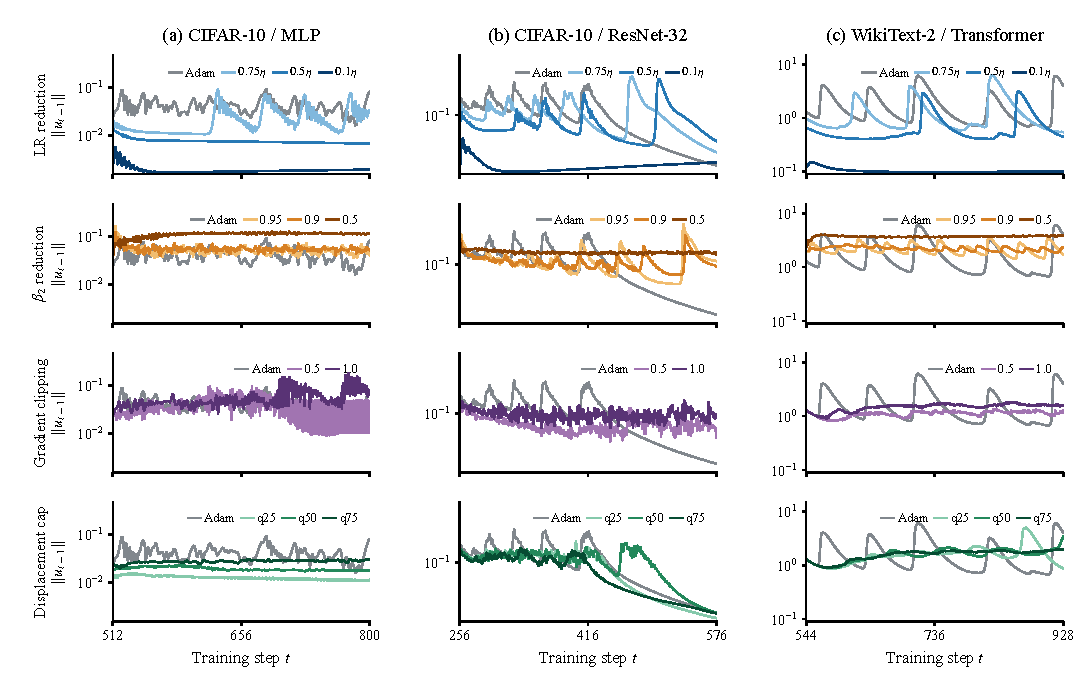
\includegraphics[width=\textwidth]{figures/a01-matched-applied-updates.pdf}
\caption{Actual applied update norms for all matched interventions. Rows correspond to immediate learning-rate reduction, late $\beta_2$ reduction, global gradient clipping, and distributed displacement caps. Gray is the same unchanged-Adam control in every row. All post-start updates are retained without smoothing; the log scale is shared across families within each model. Update $u_{t-1}$ is placed at its completed-state endpoint $t$.}
\label{fig:app-updates}
\end{figure*}

\begin{figure*}[!t]
\centering
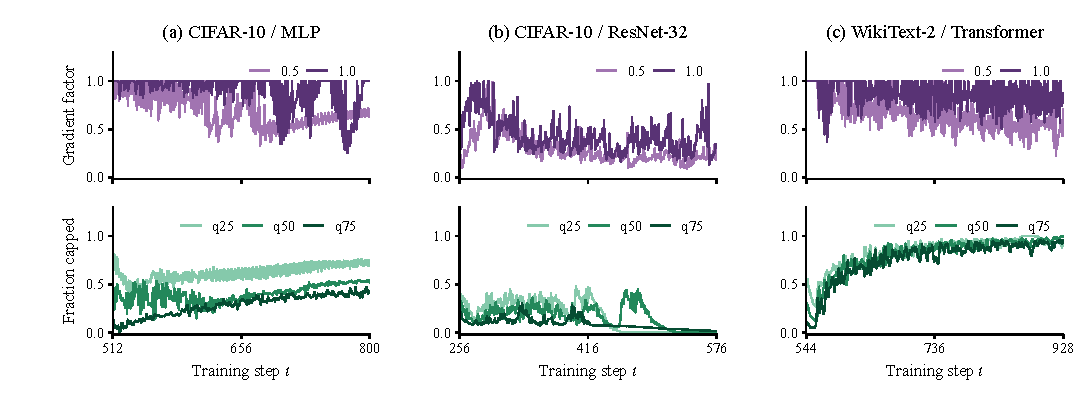
\includegraphics[width=\textwidth]{figures/a02-matched-controller-activity.pdf}
\caption{Controller activity over the same complete windows. Top: multiplicative factor retained by global gradient clipping before Adam; one means no clipping. Bottom: fraction of targeted units whose proposed increments are scaled by the displacement cap, pooled over all targeted sites; zero means no units capped. A clipping factor is not an Adam update-retention factor. All values are aligned with completed updates and unsmoothed.}
\label{fig:app-activity}
\end{figure*}

\begin{figure*}[!t]
\centering
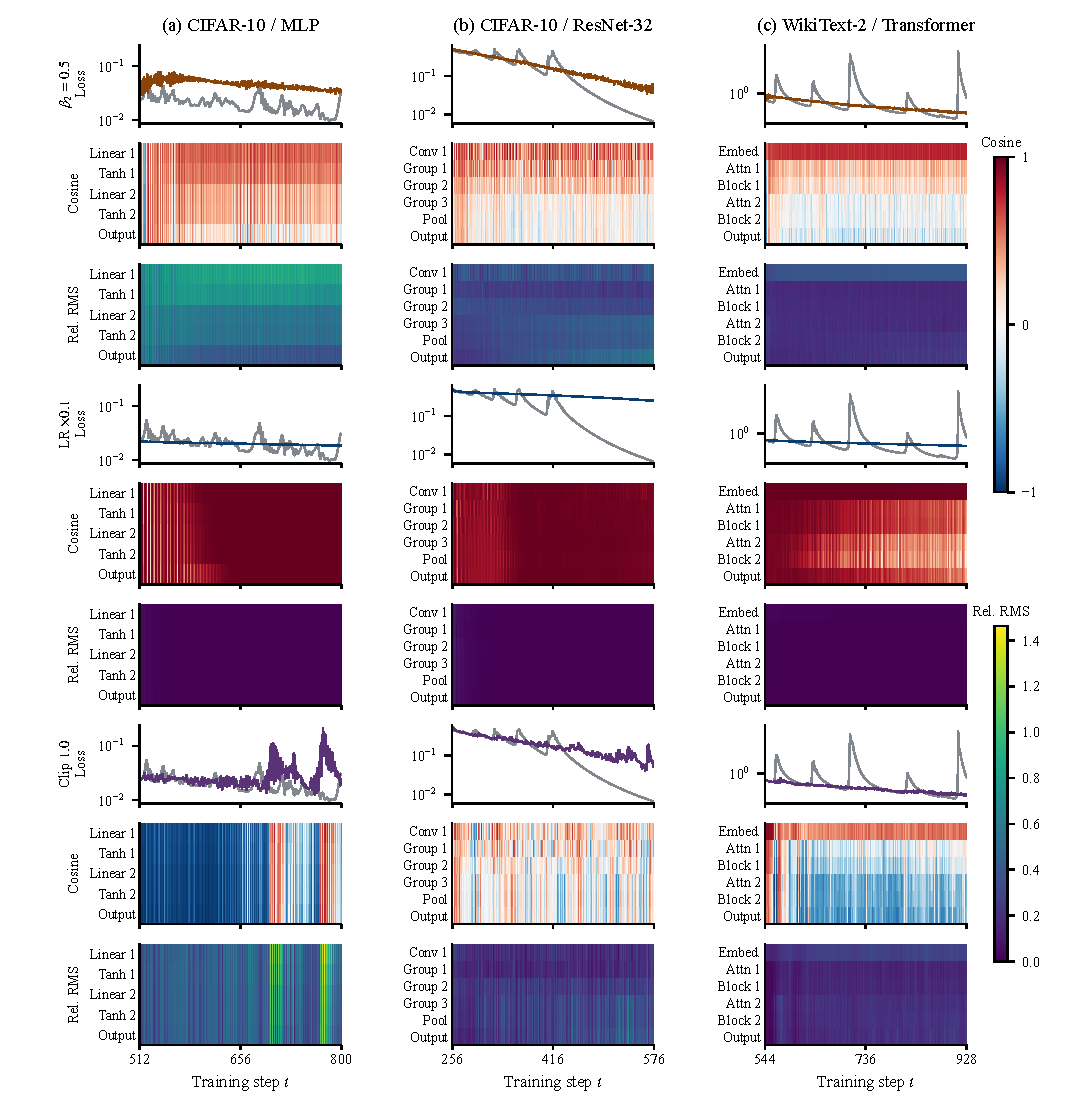
\includegraphics[width=\textwidth]{figures/a03-selected-intervention-motion.pdf}
\caption{Selected conventional interventions across the three models: $\beta_2=0.5$ (top block), LR $\times0.1$ (middle), and clip threshold 1.0 (bottom). Each block shows full training loss, consecutive representation-change cosine, and relative RMS displacement. Gray loss curves are unchanged Adam; colored curves and all heatmaps belong to the selected intervention. No Adam heatmaps are repeated. Log-loss limits are shared across the three blocks within each model. RMS uses each site's unchanged-Adam maximum as a common denominator, with one color scale across all selected settings and models; values above one exceed that baseline maximum. Every post-start change is retained, without smoothing, layer averaging, or peak markers. Sites match Fig.~\ref{fig:trace-motion}.}
\label{fig:app-selected}
\end{figure*}
\clearpage
% Reset column height after the full-width float pages before the bibliography.
\onecolumn\twocolumn
